%%%%%%%%%%%%%%%%%%%%%%%%%%%%%%%%%%%%%%%%%%%%%%%%%%%%%%%%%%%%%%%%%%%%%%%%%%%%%%%
\chapter{Introdução}
%%%%%%%%%%%%%%%%%%%%%%%%%%%%%%%%%%%%%%%%%%%%%%%%%%%%%%%%%%%%%%%%%%%%%%%%%%%%%%%

Os algoritmos deste capítulo resolvem o {\bf problema de ordenação}:
\begin{itemize}
\item {\bf Entrada}: uma sequência de $n$ números $\langle a_1, a_2, ..., a_n \rangle$.

\item {\bf Saída}:  Uma permutação $\langle {a'}_1, {a'}_2, ..., {a'}_n \rangle$ da
entrada tal que ${a'}_1 \leq {a'}_2 \leq ... \leq {a'}_n$.
\end{itemize}
Ordenação pode ser usado em diversos outros algoritmos.
Ela pode ser necessária devido a requisitos do usuário, ou para a otimização de pesquisa 
como na pesquisa binária.

Em geral os dados são mantidos em um vetor onde cada objeto possui um
atributo \textbf{chave} que deve ser mantido ordenado.
Para fins de exemplo, utiliza-se números inteiros como elementos.

Um algoritmo de ordenação possui duas características principais:
\begin{itemize}
\item {\bf Estabilidade} -- relativo a manutenção da ordem original dos itens 
com chaves iguais.
	\begin{itemize}
	\item Um algoritmo de ordenação é {\bf estável} se a ordem relativa dos itens
		com chaves iguais não se altera durante a ordenação.
	\end{itemize}
\item {\bf Uso de memória} -- quanto ao uso de memória pelo algoritmo.
	\begin{itemize}
	\item {\bf Com cópia de dados} -- utiliza um vetor temporário para realizar a ordenação. As trocas são feitas entre o vetor original e o temporário.
	\item {\bf In-place} -- as trocas são feitas dentro do próprio vetor original.
	\end{itemize}
\end{itemize}

O critério de avaliação, sendo $n$ o número de registros, pode ser por:
\begin{itemize}
\item $C(n)$ -- número de comparações.
\item $M(n)$ -- número de movimentações de elementos.
\end{itemize}
Em grande parte dos casos, nos concentramos no número de comparações.

Os métodos de ordenação podem ser {\bf interno} (em memória primária) ou {\bf externo} (em memória secundária).
Na {\bf interna} o arquivo de entrada cabe todo na memória principal, enquanto
que na {\bf externa} o arquivo não cabe na memória principal. 

A maioria dos métodos é baseada em {\bf comparações} de chaves.
Porém, existem outros métodos que utilizam o principio da {\bf distribuição}. 
Um exemplo é ordenar um baralho com 52 cartas na ordem numérica e ordem de naipes.
O algoritmo seria:
\begin{enumerate}
\item Distribuir cartas em treze montes: ases, dois, três, ...., reis.
\item Coletar os montes na ordem especificada.
\item Distribuir novamente as cartas em quatro montes: paus, ouros, copas e espadas.
\item Coletar os montes na ordem especificada.
\end{enumerate}
Alguns desses métodos são o {\bf radixsort} e o {\bf bucketsort}.

%%%%%%%%%%%%%%%%%%%%%%%%%%%%%%%%%%%%%%%%%%%%%%%%%%%%%%%%%%%%%%%%%%%%%%%%%%%%%%%
\chapter{Classificação em memória primária}
%%%%%%%%%%%%%%%%%%%%%%%%%%%%%%%%%%%%%%%%%%%%%%%%%%%%%%%%%%%%%%%%%%%%%%%%%%%%%%%

Podem ser classificados como:
\begin{itemize}
\item {\bf Métodos simples} -- adequado para vetores pequenos, requerem $O(n^2)$ comparações.
Ex.: bolha, inserção, seleção, shellsort.
\item {\bf Métodos eficientes} -- adequados para vetores grandes, requerem $O(n \log n)$ comparações.
Ex.: quicksort, mergesort, heapsort.
\item {\bf Métodos mais eficientes} -- ou por distribuição, requerem $O(n)$ atribuições. Ex.: radixsort.
\end{itemize}

%%%%%%%%%%%%%%%%%%%%%%%%%%%%%%%%%%%%%%%%%%%%%%%%%%%%%%%%%%%%%%%%%%%%%%%%%%%%%%%
\section{Métodos de ordenação simples}
%%%%%%%%%%%%%%%%%%%%%%%%%%%%%%%%%%%%%%%%%%%%%%%%%%%%%%%%%%%%%%%%%%%%%%%%%%%%%%%

%%%%%%%%%%%%%%%%%%%%%%%%%%%%%%%%%%%%%%%%%%%%%%%%%%%%%%%%%%%%%%%%%%%%%%%%%%%%%%%
\subsection{Bolha (\emph{bubble sort})}

O bubblesort ordena os elementos ao colocar o maior sempre no fim do vetor.
O algoritmo é ilustrado na figura~\ref{aula03:algo:bubblesort}.
\begin{figure}[!htb]
\centering
\begin{framed}
\begin{lstlisting}
void Bubblesort( int *A, int n ){
	int i;
	bool trocado;
	do{
		trocado = false;
		for( i = 1; i < n; i++){
			if( A[i-1] > A[i] ){
				troca( A[i-1], A[i] );
				trocado = true;
			}
		}
	} while(trocado);
}
\end{lstlisting}
\end{framed}
\caption{Algoritmo do bubblesort.}
\label{aula03:algo:bubblesort}
\end{figure}

\todo[inline]{Exemplo com $4, 9, 2, 1, 5$.}

O número de comparações é $(n-1)+(n-2)+....+2+1$ com complexidade (para pior caso)
\begin{equation*}
C(n) = \sum_{k=1}^{n-1} i = \frac{n(n-1)}{2} = O(n^2).
\end{equation*}

As principais vantagens:
\begin{itemize}
\item Algoritmo simples.
\item Algoritmo estável.
\end{itemize}

%%%%%%%%%%%%%%%%%%%%%%%%%%%%%%%%%%%%%%%%%%%%%%%%%%%%%%%%%%%%%%%%%%%%%%%%%%%%%%%
\subsection{Seleção (\emph{selection sort})}

O selectionsort coloca o menor elemento sempre no começo do vetor.
O algoritmo é ilustrado na figura~\ref{aula03:algo:selection}.
\begin{figure}[!htb]
\centering
\begin{framed}
\begin{lstlisting}
void Selecao( int *A, int n ){
	int i, j, min;
	for( i = 0; i < n; i++){
		min = i;
		for(j= i+1; j < n; j++)
			if( A[j] < A[min] )
				min = j;
		troca( A[min], A[i] );
	}
}
\end{lstlisting}
\end{framed}
\caption{Algoritmo de ordenação por seleção.}
\label{aula03:algo:selection}
\end{figure}

\todo[inline]{Exemplo com $4, 9, 2, 1, 5$.}

O número de comparações é $(n-1)+(n-2)+....+2+1$ com complexidade (qualquer caso)
\begin{equation*}
C(n) = \sum_{k=1}^{n-1} i = \frac{n(n-1)}{2} = O(n^2).
\end{equation*}

Vantagens:
\begin{itemize}
\item custo linear para movimentações.
\item interessante para vetores pequenos.
\end{itemize}
Desvantagens:
\begin{itemize}
\item vetor ordenado não ajuda, pois o custo continua quadrático.
\item algoritmo {\bf não é estável}.
\end{itemize}

%%%%%%%%%%%%%%%%%%%%%%%%%%%%%%%%%%%%%%%%%%%%%%%%%%%%%%%%%%%%%%%%%%%%%%%%%%%%%%%
\subsection{Inserção (\emph{insertion sort})}

A figura~\ref{aula02:algo:insertion} da seção~\ref{aula02:sec:insertion} ilustra
o algoritmo.
%
O número de comparações é $(n-1)+(n-2)+....+2+1$ no pior caso (ordem reversa), com complexidade
\begin{equation*}
C(n) = \sum_{k=1}^{n-1} i = \frac{n(n-1)}{2} = O(n^2).
\end{equation*}
Por outro lado, o número de comparações no melhor caso (vetor ordenado) é 
$1 + 1 + 1 + 1+ .... + 1 = n-1$ com complexidade
\begin{equation*}
C(n) = n - 1  = O(n).
\end{equation*}

\todo[inline]{Exemplo com $4, 9, 2, 1, 5$.}

Vantagens:
\begin{itemize}
\item ideal quando o vetor está ``quase'' ordenado.
\item ordenação estável.
\end{itemize}
Desvantagens:
\begin{itemize}
\item custo médio é quadratico.
\item alto custo para inserir elemento na posição correta.
\end{itemize}

%%%%%%%%%%%%%%%%%%%%%%%%%%%%%%%%%%%%%%%%%%%%%%%%%%%%%%%%%%%%%%%%%%%%%%%%%%%%%%%
\subsection{Shellsort}

Proposto por Shell em 1959, o algoritmo é uma extensão do insertion sort.
Ele é eficiente quando a entrada está parcialmente ordenado.
Porém, ele é  ineficiente no caso geral pois troca os valores apenas uma posição por vez.

A proposta geral do shellsort é trocar elementos de posições distantes para vetores muito
desordenados, e trocar elementos próximos para entradas parcialmente ordenados.
O algoritmo é ilustrado na figura~\ref{aula03:algo:shellsort}.
Quando $h = 1$ shellsort corresponde ao algoritmo de inserção.
\begin{figure}[!htb]
\centering
\begin{framed}
\begin{lstlisting}
void Shellsort( int *A, int n ){
	int i, j;
	int h = 1;
	while( h < n/3 )
		h = 3*h + 1;
	while( h >= 1 ) {
		for( i = h; i < n; i++ ){
		  for( j = i; j >= h && A[j] < A[j-h]; j -= h )
	  		  troca( A[j], A[j-h] );
		}
		h = h/3;
	}
}
\end{lstlisting}
\end{framed}
\caption{Algoritmo de ordenação Shellsort.}
\label{aula03:algo:shellsort}
\end{figure}

\todo[inline]{Exemplo com $4, 9, 2, 1, 5$, para $i= 3$, $i = 2$, e $i = 1$.}

A eficiência depende do intervalo (gap) usado. Exemplos:
\begin{itemize}
\item $gap = \frac{n}{2^k} = \frac{n}{2}, \frac{n}{4}, ...., 1 = O(n^2)$ .
\item $gap = 2^k - 1 = 1,3,7,15,31,.... = O(n^{\frac{3}{2}})$.
\end{itemize}

Vantagens:
\begin{itemize}
\item podem ser mais eficiente que os demais algoritmos de ordem quadrática.
\end{itemize}
Desvantagens:
\begin{itemize}
\item {\bf não é estável}.
\end{itemize}


%%%%%%%%%%%%%%%%%%%%%%%%%%%%%%%%%%%%%%%%%%%%%%%%%%%%%%%%%%%%%%%%%%%%%%%%%%%%%%%
\subsection{Comparação dos métodos simples}

A tabela~\ref{aula03:tab:caso01} sumariza os métodos simples e suas complexidades.
%
\begin{table}[!ht]
\centering
\caption{Comparação dos métodos simples.}
\begin{tabular}{lccccc}
\hline
          & Melhor caso & Caso médio & Pior caso & Memória & Estável \\ \hline
Bubble    & $O(n)$ & $O(n^2)$ & $O(n^2)$ & $1$ & sim \\ \hline
Selection & $O(n^2)$ & $O(n^2)$ & $O(n^2)$ & $1$ & não  \\ \hline
Insertion & $O(n)$ & $O(n^2)$ & $O(n^2)$ & $1$ &  sim \\ \hline
Shellsort & $O(n)$ & $O(n^{\frac{3}{2}})$ & $O(n^{\frac{3}{2}})$ &  $1$ & não \\ \hline
\end{tabular}
\label{aula03:tab:caso01}
\end{table}

%%%%%%%%%%%%%%%%%%%%%%%%%%%%%%%%%%%%%%%%%%%%%%%%%%%%%%%%%%%%%%%%%%%%%%%%%%%%%%%
\section{Métodos eficientes}

Os métodos eficientes são baseados na estratégia de {\bf divisão e conquista} (D\&C)
onde:
\begin{itemize}
\item {\bf divisão} -- divide um problema maior em problemas menores (subproblemas) 
recursivamente até que não seja mais possível dividir (caso base).

\item {\bf conquista} -- a solução dos problemas menores leva a solução do problema maior.
\end{itemize}

Diversos métodos de ordenação aplicam divisão e conquista. Os algoritmos detalhados
aqui são o \emph{quicksort} e o \emph{mergesort}.

%%%%%%%%%%%%%%%%%%%%%%%%%%%%%%%%%%%%%%%%%%%%%%%%%%%%%%%%%%%%%%%%%%%%%%%%%%%%%%%
\subsection{Quicksort}

Proposto em 1960 e publicado em 1962, a ideia básica é dividir o problema de
ordenar um conjunto com $n$ itens em dois problemas menores.
Os problemas menores são ordenados independentemente, e combinados para
produzir a solução final.

O Quicksort funciona da seguinte forma:
\begin{enumerate}
\item selecionar um elemento como {\bf pivô}.
\item particionar os elementos em dois subvetores:
	\begin{enumerate}
	\item elementos menores que o pivô.
	\item elementos maiores que o pivô.
	\end{enumerate}
\item executar o quicksort recursivamente em cada subvetor.
\end{enumerate}

Os passos do {\bf particionamento} são:
\begin{enumerate}
\item escolher um {\bf pivô} $pivo$.
\item percorrer o vetor a partir da esquerda até que $A[esq] \geq pivo$.
\item percorrer o vetor a partir da direita até que $A[dir] \leq pivo$.
\item trocar $A[esq]$ com $A[dir]$.
\item continuar até que $esq$ e $dir$ se cruzem, ou seja, enquanto $esq >= dir$.
\end{enumerate}

\todo[inline]{Exemplo com $40, 20, 10, 80, 60, 50, 7, 30, 100$.}

O algoritmo do Quicksort é ilustrado na figura~\ref{aula03:algo:quicksort}
enquanto que o particionamento na figura~\ref{aula03:algo:partition}.
Nota-se que o pivô escolhido em cada particionamento é o número 
na primeira posição do subvetor (linha 4).
%
\begin{figure}[!htb]
\centering
\begin{framed}
\begin{lstlisting}
void Quicksort( int *A, int esq, int dir ){
	int i;
	if( esq < dir ){
		i = Partition( A, esq, dir );
		Quicksort( A, esq, i - 1 );
		Quicksort( A, i + 1, dir );
	}
}
\end{lstlisting}
\end{framed}
\caption{Algoritmo de ordenação Quicksort.}
\label{aula03:algo:quicksort}
\end{figure}

\begin{figure}[!htb]
\centering
\begin{framed}
\begin{lstlisting}
int Partition( int *A, int inicio, int fim ){
	int esq = inicio;
	int dir = fim + 1;
	int pivo = A[inicio];
	do {
		while( pivo > A[++esq] )
			if( esq == fim ) break;
		while( pivo < A[--dir] )
			if( dir == inicio ) break;
		if( esq < dir )
			troca( &A[esq], &A[dir] );
	} while( esq < dir  );
	troca( &A[inicio], &A[dir] );
	return dir;
}
\end{lstlisting}
\end{framed}
\caption{Algoritmo de partição do Quicksort.}
\label{aula03:algo:partition}
\end{figure}

A análise do Quicksort depende da {\bf escolha do pivô} para balanceamento do
particionamento, essencial na eficiencia do algoritmo.

O melhor caso do Quicksort acontece quando os dois subvetores possuem tamanho
$n/2$ e aplica-se Quicksort recursivamente.
Dado sua estrutura de árvore, a altura da árvore será $O(\log n)$ e o número
de comparações em cada nível da árvore é $O(n)$. 
Logo, o custo no {\bf melhor caso} é $O(n \log n)$.

Para o pior caso, vamos supor que o pivô é o primeiro elemento e que o vetor já esta 
ordenado.  
O particionamento resulta em subvetores de tamanho $1$ e $n-1$ onde executa-se Quicksort
em ambos recursivamente.
Dessa forma, a altura da árvore é $O(n)$ (pode-se imaginar todos os nós com 1 filho)
e comparações por nível de $O(n)$.
O custo no {\bf pior caso} será $O(n^2)$.

O problema do pior caso no Quicksort pode ser contornado ao escolher o ponto médio
de três elementos do vetor.
Por exemplo, das posições $A[0]$, $A[n/2]$ e $A[n-1]$, escolhe-se o que tem
valor médio entre eles.

%%%%%%%%%%%%%%%%%%%%%%%%%%%%%%%%%%%%%%%%%%%%%%%%%%%%%%%%%%%%%%%%%%%%%%%%%%%%%%%
\subsection{Mergesort}

A ideia do Mergesort é dividir um conjunto com $n$ itens em duas partes iguais.
Os problemas menores são ordenados independentemente, e mesclados para
produzir a solução final.

O algoritmo do Mergesort é ilustrado na figura~\ref{aula03:algo:mergesort}
enquanto que a mescla na figura~\ref{aula03:algo:merge}.
%
\begin{figure}[!htb]
\centering
\begin{framed}
\begin{lstlisting}
void Mergesort( int *A, int inicio, int fim, int *aux ){
	int meio;
	if( inicio < fim ){
		meio = (inicio + fim - 1)/2;
		Mergesort( A, inicio, meio, aux );
		Mergesort( A, meio + 1, fim, aux );
		Merge( A, inicio, meio, fim, aux );
	}
}
\end{lstlisting}
\end{framed}
\caption{Algoritmo de ordenação Mergesort.}
\label{aula03:algo:mergesort}
\end{figure}

\begin{figure}[!htb]
\centering
\begin{framed}
\begin{lstlisting}
void Merge( int *A, int inicio, int meio, int fim, int *aux ){
	int i = inicio, j = meio + 1, k;
	for(k = inicio; k <= fim; k++ )
		aux[k] = A[k];
	for(k = inicio; k <= fim; k++ ){
		if(i > meio)		 A[k] = aux[j++];
		else if(j > fim)	 A[k] = aux[i++];
		else if(aux[j] < aux[i]) A[k] = aux[j++];
		else 			 A[k] = aux[i++];
	}
}
\end{lstlisting}
\end{framed}
\caption{Algoritmo para mesclar subvetores do Mergesort.}
\label{aula03:algo:merge}
\end{figure}

O algoritmo de Mergesort ilustrado {\bf não é in-place} e utiliza um vetor
temporário (ou auxiliar) para a operação de mescla.
Dessa forma, pode-se mesclar os elementos no vetor temporário e depois copiar
de volta ao vetor original.
O uso do vetor auxiliar simplifica o algoritmo, mas necessita do dobro de
espaço para fazer a ordenação.

A análise do Mergesort deve considerar que ele divide o problema em dois
subvetores de tamanho $n/2$ e aplica Mergesort recursivamente.
O custo de comparações em cada nível é $cn$ sendo o primeiro nível
$c(n/2)+c(n/2)$, o segundo $c(n/4)+c(n/4)+c(n/4)+c(n/4)$, etc.
A árvore de recursão terá $\log n + 1$ níveis, cada um com custo $cn$.
Portanto, o custo total será $cn(\log n + 1) = cn \log n + cn$.
O custo no {\bf pior caso} do algoritmo é $O(n \log n)$.

No melhor caso, o vetor de entrada já está ordenado. 
Uma forma eficiente de descobrir é testar o último elemento do primeiro subvetor
e o primeiro elemento do segundo subvetor.
As chamadas recursivas ainda são necessárias mas não será preciso fazer chamadas
ao Merge.
O custo no {\bf melhor caso} é $O(n)$.

%%%%%%%%%%%%%%%%%%%%%%%%%%%%%%%%%%%%%%%%%%%%%%%%%%%%%%%%%%%%%%%%%%%%%%%%%%%%%%%
\subsection{Heapsort}

Heapsort possue o mesmo princípio da ordenação por seleção onde:
\begin{enumerate}
\item selecionar o maior item do vetor.
\item trocar com o item da primeira posição do vetor.
\item repetir essa operação para os $n-1$ elementos, os $n-2$, e assim sucessivamente.
\end{enumerate}
O custo de encontrar o menor elemento é de $n-1$ comparações, porém esse custo pode ser reduzido
com uma estrutura de dados {\bf heap}.

\subsubsection*{Definição de heap}

O heap é uma árvore binária balanceada e justificada a esquerda onde todos os
nós satisfazem a {\bf propriedade do heap}: seu valor é menor ou igual ao valor
do nó pai.
Uma árvore balanceada significa que todos os níveis estão completos com exceção
do nível folha.
Uma árvore justificada a esquerda significa que os nós do último nível
estão mais a esquerda possível.
A partir da propriedade do heap, conclui-se que o maior elemento de todos
na árvore está no topo.

A inserção no heap sempre ocorre no último nível, a direita do último nó.
Se o último nível estiver cheio, começa um novo nível. 
Na remoção o elemento removido é trocado pelo mais a direita da árvore.
As operações de inserção e remoção podem fazer com que a árvore perca a
propriedade do heap.  A correção é feita por transformações locais, com a troca
do nó pai pelo nó filho de maior valor.

Heaps podem ser mapeados para vetores com operações sobre vetores.
No caso de um nó de indice $i$:
\begin{itemize}
\item o filho à {\bf esquerda} está em $2*i+1$.
\item o filho à {\bf direita} está em $2*i+2$.
\end{itemize}
A {\bf raiz} é o primeiro elemento do vetor e o nó mais à direita é o último
elemento do vetor.
A figura~\ref{aula03:fig:heap} ilustra um exemplo de vetor e seu heap correspondente.
%
\begin{figure}[ht]
\centering
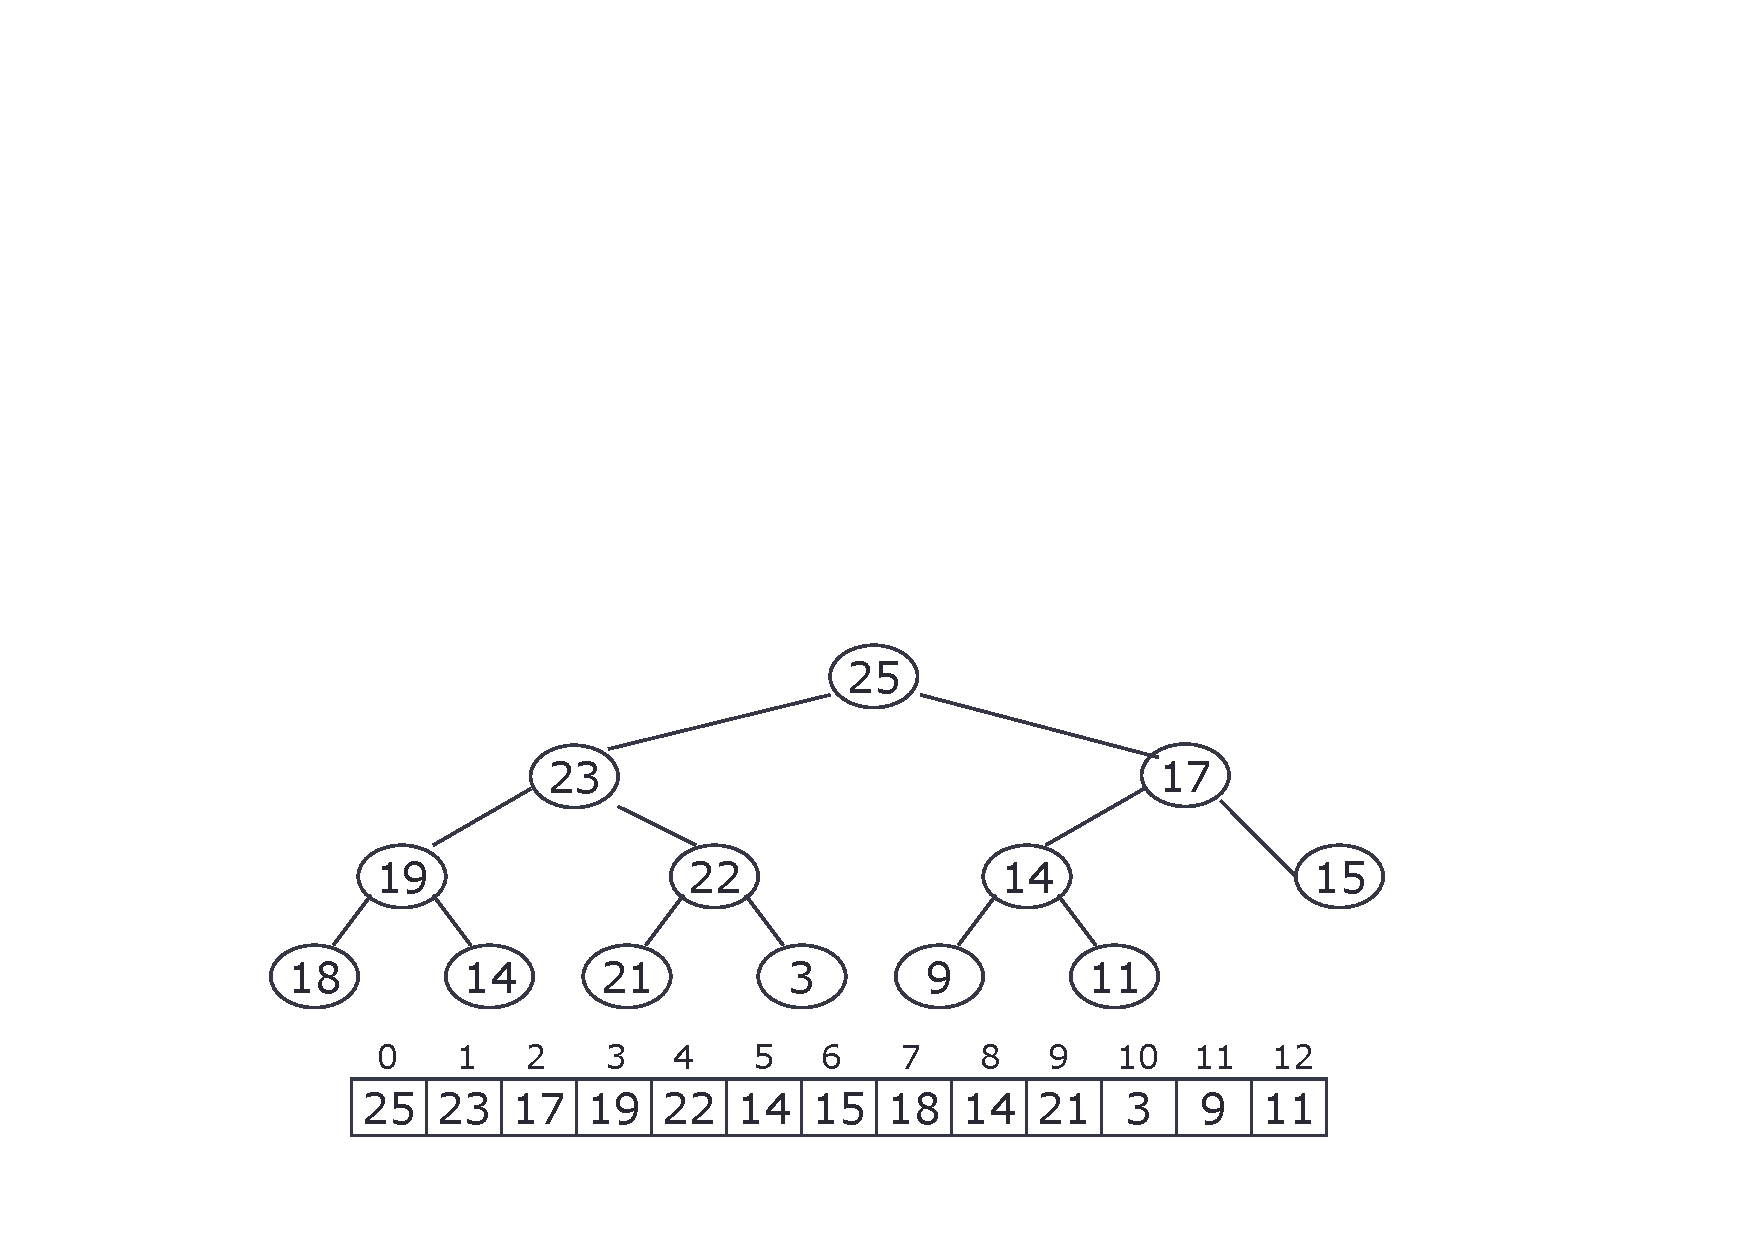
\includegraphics[width=0.8\textwidth]{heap}
\caption{Exemplo de vetor e representação como um heap.}
\label{aula03:fig:heap}
\end{figure}

\subsubsection*{Heap para ordenação}

O primeiro algoritmo (figura~\ref{aula03:algo:heap:refaz}) garante a principal
propriedade do heap a partir de uma posição $i$ do vetor.
%
\begin{figure}[!htb]
\centering
\begin{framed}
\begin{lstlisting}
void Refaz( int *A, int i, int n ){
	int esq = 2 * i + 1;
	int dir = 2 * i + 2;
	int maior;

	if( esq < n && A[esq] > A[i] )     maior = esq;
	else                               maior = i;
	if( dir < n && A[dir] > A[maior] ) maior = dir;

	if( maior != i ){
		troca( &A[i], &A[maior] );
		Refaz( A, maior, n );
	}
}
\end{lstlisting}
\end{framed}
\caption{Algoritmo que transforma a árvore em um heap de uma posição $i$ do vetor.}
\label{aula03:algo:heap:refaz}
\end{figure}

O segundo algoritmo (figura~\ref{aula03:algo:heap:constroi}) constroi
um heap a partir de um vetor. 
Para cada posição do vetor, ele usa a função \lstinline{Refaz()} e transforma
o vetor em um heap.
%
\begin{figure}[!htb]
\centering
\begin{framed}
\begin{lstlisting}
void Constroi( int *A, int n ){
	int k;
	for(k = n/2; k >= 0; k-- ){
		Refaz( A, k, n );
	}
}
\end{lstlisting}
\end{framed}
\caption{Algoritmo que constroi o heap de um vetor $n$.}
\label{aula03:algo:heap:constroi}
\end{figure}

O algoritmo Heapsort (figura~\ref{aula03:algo:heapsort}) inicia com a construção
de um heap com o vetor de entrada.
Como o maior elemento do heap fica na posição $A[0]$,
o algoritmo coloca o elemento no final do vetor ao trocar com $A[n-1]$.
Em seguida ele ignora o último elemento (o maior) e usa \lstinline{Refaz()} para
reconstruir o heap.
O algoritmo repete esses dois passos $n-1$ vezes.
%
\begin{figure}[!htb]
\centering
\begin{framed}
\begin{lstlisting}
void Heapsort( int *A, int n ){
	int i;
	Constroi( A, n );
	for( i = n-1; i > 0; i-- ) {
		troca( &A[0], &A[i] );
		Refaz( A, 0, i );
	}
}
\end{lstlisting}
\end{framed}
\caption{Algoritmo do Heapsort: passa o maior elemento para o fim e refaz o heap.}
\label{aula03:algo:heapsort}
\end{figure}

\subsubsection*{Análise}

A análise envolve o custo da construção do heap e da leitura dos elementos em ordem.
A construção do heap adiciona um elemento ao final e pode ser deslocado até a raiz.
Como a árvore é balanceada, o deslocamento tem custo $O(\log n)$ e 
isso é feito $n$ vezes.
O curso de construir o heap é $O(n \log n)$. 

A leitura em ordem a troca do primeiro com o último com custo $O(1)$. Após a troca,
o elemento pode precisar ser deslocado até o nível folha.
Em uma árvore balanceada o custo de mover é $O(\log n)$.
Como isso é feito $n$ vezes, o custo de leitura em ordem é $O(n \log n)$.

O custo total é $2n \log n = O(n \log n)$.

%%%%%%%%%%%%%%%%%%%%%%%%%%%%%%%%%%%%%%%%%%%%%%%%%%%%%%%%%%%%%%%%%%%%%%%%%%%%%%%
\subsection{Comparação entre métodos eficientes}

A tabela~\ref{aula03:tab:caso02} sumariza o Mergesort e Quicksort com suas complexidades.
%
\begin{table}[!ht]
\centering
\caption{Comparação dos métodos simples.}
\begin{tabular}{lccccc}
\hline
          & Melhor caso & Caso médio & Pior caso & Memória & Estável \\ \hline
Quicksort & $O(n \log n)$ & $O(n \log n)$ & $O(n^2)$ & $1$ & não \\ \hline
Mergesort & $O(n)$ & $O(n \log n)$ & $O(n \log n)$ & $n$ & sim \\ \hline
Heapsort & $O(n \log n)$ & $O(n \log n)$ & $O(n \log n)$ & $1$ & não \\ \hline
%
\end{tabular}
\label{aula03:tab:caso02}
\end{table}

Em casos típicos o Quicksort tem melhor desempenho que Heapsort,
que é melhor que Mergesort.
O Heapsort é melhor para aplicações de tempo crítico, ou ordenações parciais
(apenas 10 elementos por exemplo).

Há implementações estáveis
do Quicksort, porém o desempenho pode ser afetado.  Existem algoritmos do
Mergesort com memória in-place, mas o desempenho pode ser afetado.

%%%%%%%%%%%%%%%%%%%%%%%%%%%%%%%%%%%%%%%%%%%%%%%%%%%%%%%%%%%%%%%%%%%%%%%%%%%%%%%
\section{Métodos de ordenação por distribuição}
%%%%%%%%%%%%%%%%%%%%%%%%%%%%%%%%%%%%%%%%%%%%%%%%%%%%%%%%%%%%%%%%%%%%%%%%%%%%%%%

Os algoritmos discutidos até agora tem custo $O(n \log n)$ em casos
médios.
Porém, caso o custo de espaço não é problema e somente a comparação
lexicográfica é necessária, é possível usar estratégias sem comparação.

Os algoritmos de ordenação por distribuição distribuem os elementos de entrada
em estruturas intermediárias com base nos seus valores.
Essas estruturas, por si só, já auxiliam na ordenação dos elementos.

%%%%%%%%%%%%%%%%%%%%%%%%%%%%%%%%%%%%%%%%%%%%%%%%%%%%%%%%%%%%%%%%%%%%%%%%%%%%%%%
\subsection{Countingsort}

Countingsort assume que os elementos de entrada $n$ são inteiros e
os valores (chaves) estão no intervalo de $0$ até $k$ para um inteiro $k$.
Esse algoritmo requer um vetor de entrada $A$, um vetor de saída $B$ e um
temporário $C$ de tamanho $k$ sendo $k$ o maior valor armazenado.
O algoritmo da figura~\ref{aula03:algo:counting} mostra a implementação do
Countingsort.
%
\begin{figure}[!htb]
\centering
\begin{framed}
\begin{lstlisting}
void Countingsort( int *A, int* B, int n, int k ){
	int C[k];
	int i;

	for( i = 0; i < k; i++)    C[i] = 0;
	for( i = 0; i < n; i++)    C[A[i]]++;
	for( i = 1; i < k; i++)    C[i] = C[i] + C[i-1];
	for( i = n-1; i >= 0; i-- ){
		B[C[A[i]] - 1] = A[i];
		C[A[i]]--;
	}
}
\end{lstlisting}
\end{framed}
\caption{Algoritmo do Countingsort para $n$ elementos de valor até $k$.}
\label{aula03:algo:counting}
\end{figure}

O custo do Countingsort depende de zerar o vetor $C$ ($O(k)$), 
contar em $C$ o número de ocorrências dos valores de $A$ ($O(n)$),
somar as ocorrências ($O(k)$) e ordenar o vetor em $B$ ($O(n)$).
Assim, o custo será $k + n + k + n = O(k + n)$.
O custo em espaço é $O(n + k)$ para usar $B$ e $C$.

O Countingsort custa menos que $O(n \log n)$ porque não é um algoritmo baseado
em comparação.  Ele usa o valor dos elementos para indexar o vetor.
O algoritmo é estável e não é in-place, assim como só funciona com inteiros.

%%%%%%%%%%%%%%%%%%%%%%%%%%%%%%%%%%%%%%%%%%%%%%%%%%%%%%%%%%%%%%%%%%%%%%%%%%%%%%%
\subsection{Bucketsort}

O Bucketsort assume que a entrada está uniformemente distribuída e que tem um
tempo de execução médio de $O(n)$.
Ele assume que os números de entrada são distribuídos em um intervalo $[0,1)$ (por exemplo)
e são dividos em $r$ grupos chamados {\bf buckets}.

O algoritmo distribui os $n$ elementos entre os buckets.
Para gerar a saída, ele ordena cada bucket e depois copia para saída 
cada elemento dos buckets em ordem.

O algoritmo da figura~\ref{aula03:algo:bucket} mostra a implementação do
Bucketsort.
Ele usa $r$ como o número de buckets usados e $B[r]$ um vetor de listas para
cada bucket.
Ao distribuir os números, ele ordena cada bucket com uma função
que ordena a lista. A ordenação da lista pode ser feita por
Insertionsort.
Por fim, ele percorre cada lista para copiar os elementos na saída $A$.
%
\begin{figure}[!htb]
\centering
\begin{framed}
\begin{lstlisting}
void Bucketsort( float *A, int n, int r ){
	lista_t* B[r];
	int i, j;
	for( j = 0; j < r; j++ )    B[i] = lista_cria();
	for( i = 0; i < n; i++ ){
		int j = (int)floor(A[i]*10);
		lista_insere( B[j], A[j] );
	}
	for( j = 0; j < r; j++)    OrdenaLista(B[j]);
	i = 0;
	for( j = 0; j < r; j++){
		while(!lista_vazia(B[j]))
			A[i++] = lista_remove(B[i]);
	}
}
\end{lstlisting}
\end{framed}
\caption{Algoritmo do Bucketsort para $n$ com $k$ buckets.}
\label{aula03:algo:bucket}
\end{figure}

O custo depende do número de buckets usados. 
A distribuição é mais uniforme se os buckets serem equivalente ao número de possíveis valores.
Para uma entrada $n$ e $r$ buckets, o custo em espaço é $O(n+r)$.
Em custo, assumindo uma distribuição uniforme, tem-se $n$ cópias para os buckets, $r$ passagens pelos buckets e
$n$ cópias de volta para o vetor original.
A ordenação de cada bucket é desprezível pois contem $1$ ou poucos elementos.
O custo será $O(2n+r) = O(n+r)$.

%%%%%%%%%%%%%%%%%%%%%%%%%%%%%%%%%%%%%%%%%%%%%%%%%%%%%%%%%%%%%%%%%%%%%%%%%%%%%%%
\subsection{Radixsort}

O algoritmo da figura~\ref{aula03:algo:radix} mostra a implementação do Radixsort
para números de base 10 com 2 dígitos.
%
\begin{figure}[!htb]
\centering
\begin{framed}
\begin{lstlisting}
void Radixsort( int *A, int* B, int n, int digitos ){
	int C[10];
	int k = 10;
	int i, d;
	int base = 10;
	int div = 1;

	for(d = 1; d <= digitos; d++){
		for( i = 0; i < k; i++)    C[i] = 0;
		for( i = 0; i < n; i++)    C[ (A[i]/div)%base ]++;
		for( i = 1; i < k; i++)    C[i] = C[i] + C[i-1];
		for( i = n-1; i >= 0; i-- ){
			B[C[ (A[i]/div)%base ] - 1] = A[i];
			C[ (A[i]/div)%base ]--;
		}
		for( i = 0; i < n; i++)    A[i] = B[i];
		div = div * base;
	}
}
\end{lstlisting}
\end{framed}
\caption{Algoritmo do Radixsort para números de base 10 (2 dígitos).}
\label{aula03:algo:radix}
\end{figure}

%%%%%%%%%%%%%%%%%%%%%%%%%%%%%%%%%%%%%%%%%%%%%%%%%%%%%%%%%%%%%%%%%%%%%%%%%%%%%%%
\subsection{Comparação entre métodos por distribuição}

A tabela~\ref{aula03:tab:cmp:dist} ilustra a comparação entre os métodos onde:
\begin{itemize}
\item $n = $ número de elementos.
\item $k = $ número de valores.
\item $s = $ tamanho do alfabeto.
\end{itemize}
%
\begin{table}[!ht]
\centering
\caption{Comparação dos métodos por distribuição.}
\begin{tabular}{lccccc}
\hline
          & Melhor caso & Caso médio & Pior caso & Memória & Estável \\ \hline
Countingsort & $O(n+k)$ & $O(n+k)$ & $O(n+k)$ & $n+k$ & sim \\ \hline
Bucketsort   & $O(n+r)$ & $O(n+r)$ & $O(n^2+r)$ & $n+r$ & sim \\ \hline
Radixsort   & $O(k n)$ & $O(k n)$ & $O(k n)$ & $n+s$ & sim \\ \hline
%
\end{tabular}
\label{aula03:tab:cmp:dist}
\end{table}

%%%%%%%%%%%%%%%%%%%%%%%%%%%%%%%%%%%%%%%%%%%%%%%%%%%%%%%%%%%%%%%%%%%%%%%%%%%%%%%
\section{Comparação geral de métodos}
%%%%%%%%%%%%%%%%%%%%%%%%%%%%%%%%%%%%%%%%%%%%%%%%%%%%%%%%%%%%%%%%%%%%%%%%%%%%%%%

A tabela~\ref{aula03:tab:cmp:total} mostra uma comparação geral de métodos 
de ordenação.
%
\begin{table}[!ht]
\centering
\caption{Comparação geral dos métodos de ordenação.}
\begin{tabular}{lccccc}
\hline
          & Melhor caso & Caso médio & Pior caso & Memória & Estável \\ \hline
Quicksort & $O(n \log n)$ & $O(n \log n)$ & $O(n^2)$ & $1$ & não \\ \hline
Mergesort & $O(n)$ & $O(n \log n)$ & $O(n \log n)$ & $n$ & sim \\ \hline
Heapsort & $O(n \log n)$ & $O(n \log n)$ & $O(n \log n)$ & $1$ & não \\ \hline
Radixsort & $O(k n)$ & $O(k n)$ & $O(k n)$ & $n+s$ & sim \\ \hline
%
\end{tabular}
\label{aula03:tab:cmp:total}
\end{table}

%%%%%%%%%%%%%%%%%%%%%%%%%%%%%%%%%%%%%%%%%%%%%%%%%%%%%%%%%%%%%%%%%%%%%%%%%%%%%%%
\section{Exercícios}
%%%%%%%%%%%%%%%%%%%%%%%%%%%%%%%%%%%%%%%%%%%%%%%%%%%%%%%%%%%%%%%%%%%%%%%%%%%%%%%

\begin{enumerate}
\item Ordene os elementos $3, 7, 1, 4, 9, 2$ usando os métodos: bolha, seleção,
inserção, shellsort (com gaps $3, 2, 1$). Não esqueça de exibir o estado do vetor a cada troca
de elementos.

\item Demonstre as etapas do Quicksort para ordenar a 

\item Ordene os elementos do vetor $3, 10, 8, 9, 5, 4, 1, 2$ usando os métodos: 
Quicksort (primeiro elemento como pivô) e Mergesort. Exibir o estado do vetor toda vez que ocorrer 
uma troca.

\item Ordene o vetor $5, 3, 17, 10, 8, 9$ usando Heapsort.
\end{enumerate}
